\documentclass{article}
\usepackage[a4paper,top=3cm,bottom=2.5cm,left=2.5cm,
            right=2cm,marginparwidth=1.75cm,
            headheight=5pt]{geometry}
\usepackage[T5]{fontenc}
\usepackage[utf8]{inputenc}
\usepackage[document]{ragged2e}
\usepackage[vietnamese]{babel}
\usepackage[unicode]{hyperref}
\usepackage{amsmath}
\usepackage{setspace}
\usepackage{graphicx}
\usepackage{caption}
\usepackage{subcaption}
\usepackage{tcolorbox}
\usepackage{listings}
\usepackage{hyperref}
\usepackage{xcolor}
\usepackage{longtable}
\usepackage{titlesec}
\usepackage{floatrow}
\usepackage[nottoc]{tocbibind}
\usepackage{mdframed}
\usepackage{amsmath}
\usepackage{amssymb}
\usepackage{tgbonum}
\usepackage{type1cm}
\usepackage{indentfirst}
\usepackage{lettrine}
\usepackage{colortbl}
\usepackage{fancyhdr}
\usepackage{wrapfig}
\usepackage{lastpage}
\usepackage{url}
\addto\captionsenglish{
  \renewcommand{\contentsname}{MỤC LỤC}%
  \renewcommand{\listfigurename}{Danh sách ảnh}%
  \renewcommand{\listtablename}{Danh sách bảng}%
  \renewcommand{\figurename}{Hình}
  \renewcommand{\tablename}{Bảng}
}
\pagestyle{fancy}
\fancyhf{}
\rhead{Toán ứng dụng và thống kê}
\lhead{\color{cyan}Đồ án 2: Image Processing}
\lfoot{Trang \thepage /\pageref{LastPage}}
\renewcommand{\footrulewidth}{0.4pt}
\setlength{\parindent}{5pt}
\setlength{\parskip}{1cm}
\renewcommand{\baselinestretch}{1.5}
\newmdenv[linecolor=black,skipabove=\topsep,skipbelow=\topsep,
leftmargin=2.5cm,rightmargin=2.5cm,
innerleftmargin=5cm,innerrightmargin=5cm]{mybox}
\usepackage{multicol}
\usepackage{indentfirst}
\usepackage{color}
\usepackage{apacite}
\usepackage{tikz}
\graphicspath{{Figures/}} 
\usepackage[square, numbers, comma, sort&compress]{natbib}  
\usepackage{lipsum}
\usetikzlibrary{calc}
\setlength{\columnseprule}{2pt}
\def\columnseprulecolor{\color{black}}
\def\maru#1{\textcircled{\scriptsize#1}}

\begin{document}
% Bìa trang
\begin{titlepage}
\begin{tikzpicture}[remember picture,overlay,inner sep=0,outer sep=0]
     \draw[blue!70!black,line width=4pt] ([xshift=-1.5cm,yshift=-2cm]current page.north east) coordinate (A)--([xshift=2cm,yshift=-2cm]current page.north west) coordinate(B)--([xshift=2cm,yshift=2cm]current page.south west) coordinate (C)--([xshift=-1.5cm,yshift=2cm]current page.south east) coordinate(D)--cycle;

     \draw ([yshift=0.5cm,xshift=-0.5cm]A)-- ([yshift=0.5cm,xshift=0.5cm]B)--
     ([yshift=-0.5cm,xshift=0.5cm]B) --([yshift=-0.5cm,xshift=-0.5cm]B)--([yshift=0.5cm,xshift=-0.5cm]C)--([yshift=0.5cm,xshift=0.5cm]C)--([yshift=-0.5cm,xshift=0.5cm]C)-- ([yshift=-0.5cm,xshift=-0.5cm]D)--([yshift=0.5cm,xshift=-0.5cm]D)--([yshift=0.5cm,xshift=0.5cm]D)--([yshift=-0.5cm,xshift=0.5cm]A)--([yshift=-0.5cm,xshift=-0.5cm]A)--([yshift=0.5cm,xshift=-0.5cm]A);


     \draw ([yshift=-0.3cm,xshift=0.3cm]A)-- ([yshift=-0.3cm,xshift=-0.3cm]B)--
     ([yshift=0.3cm,xshift=-0.3cm]B) --([yshift=0.3cm,xshift=0.3cm]B)--([yshift=-0.3cm,xshift=0.3cm]C)--([yshift=-0.3cm,xshift=-0.3cm]C)--([yshift=0.3cm,xshift=-0.3cm]C)-- ([yshift=0.3cm,xshift=0.3cm]D)--([yshift=-0.3cm,xshift=0.3cm]D)--([yshift=-0.3cm,xshift=-0.3cm]D)--([yshift=0.3cm,xshift=-0.3cm]A)--([yshift=0.3cm,xshift=0.3cm]A)--([yshift=-0.3cm,xshift=0.3cm]A);

   \end{tikzpicture}
\newcommand{\HRule}{\rule{\linewidth}{0.5mm}}
\center

\textsc{\Large TRƯỜNG ĐẠI HỌC KHOA HỌC TỰ NHIÊN}\\[0.5cm]
\textsc{\Large KHOA CÔNG NGHỆ THÔNG TIN}\\[1cm]

\includegraphics[width=0.3\textwidth]{logo/KHTN.jpg}\\[1cm]

\HRule \\[0.4cm]
{\huge \bfseries ĐỒ ÁN 2: IMAGE PROCESSING} \\[0.4cm]
{\large TOÁN ỨNG DỤNG VÀ THỐNG KÊ}\\[0.1cm]
\HRule \\[1.5cm]

\centerline{\Large{\textbf{Triệu Nhật Minh — 21127112 — 21CLC02}}}
\vspace{2.5cm}
\centerline{\large{\textit{Giảng viên hướng dẫn}}}
\vspace{0.25cm}
\centerline{\large{Vũ Quốc Hoàng}}
\centerline{\large{Lê Thanh Tùng}}
\centerline{\large{Nguyễn Văn Quang Huy}}
\centerline{\large{Phan Thị Phương Uyên}}

\vspace{2.5cm}
\centerline{\today}


\vfill % Wipe blank space of the page.
\end{titlepage}

% Mục lục tự động
\setlength{\parskip}{.7em}
\tableofcontents
\newpage

% Table of Figures & Tables
\setlength{\parskip}{.5em}
%\listoffigures
%\listoftables
\newpage

% Bắt đầu nội dung
\section{Hướng dẫn sử dụng}
\begin{description}
  \item[Bước 1:] Run all các cell trong notebook \textbf{21127112.ipynb} (hoặc chỉ run cell cuối cùng để chạy hàm main nếu đã khởi chạy các hàm bổ trợ từ trước).
  \item[Bước 2: ] Nhập đường dẫn tới ảnh cần xử lý (chỉ cần tên ảnh nếu ảnh đã nằm cùng thư mục với notebook).
  \item[Bước 3: ] Chọn chức năng cần thực hiện (từ 0-8 tương ứng với các chức năng và 9 để thoát chương trình).
  \item[Bước 4: ] 
\end{description}

\section{Đánh giá kết quả}
\begin{longtable}[c]{|r|l|c|l|}
  \hline
  \rowcolor[HTML]{00D2CB} 
  \multicolumn{1}{|c|}{\cellcolor[HTML]{00D2CB}{\color[HTML]{FFFFFF} \textbf{STT}}} & \multicolumn{1}{c|}{\cellcolor[HTML]{00D2CB}{\color[HTML]{FFFFFF} \textbf{Chức năng}}} & {\color[HTML]{FFFFFF} \textbf{Mức độ hoàn thành}} & \multicolumn{1}{c|}{\cellcolor[HTML]{00D2CB}{\color[HTML]{FFFFFF} \textbf{Kết quả}}} \\ \hline
  \endfirsthead
  %
  \endhead
  1 & Thay đổi độ sáng cho ảnh & 100\% & \parbox[c]{8em}{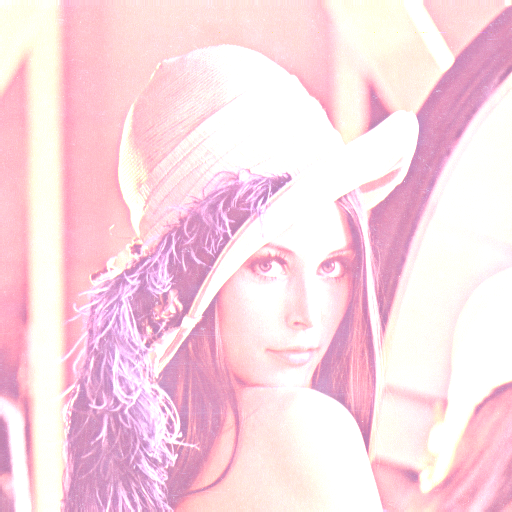
\includegraphics[width=8em]{image/Lenna_brightness_128.png}} \\ \hline
  2 & Thay đổi độ tương phản & 100\% & \parbox[c]{8em}{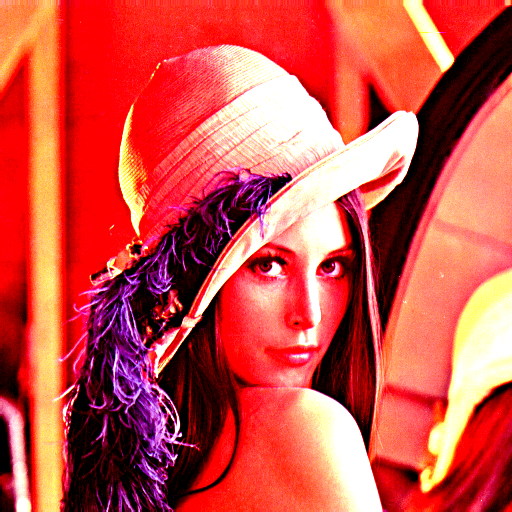
\includegraphics[width=8em]{image/Lenna_contrast_128.png}} \\ \hline
  3 & Lật ảnh ngang & 100\% & \parbox[c]{8em}{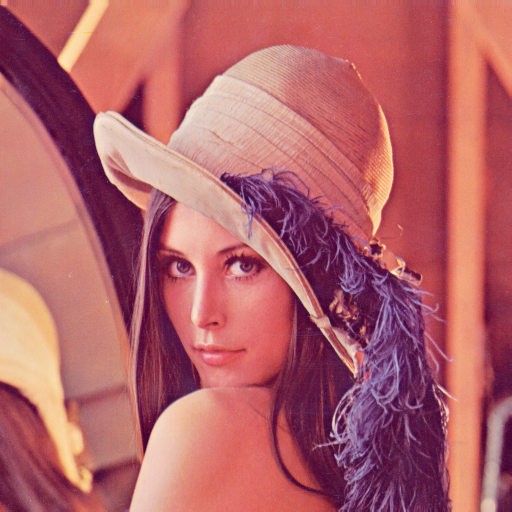
\includegraphics[width=8em]{image/Lenna_flip_horizontal.png}} \\ \hline
  4 & Lật ảnh dọc & 100\% & \parbox[c]{8em}{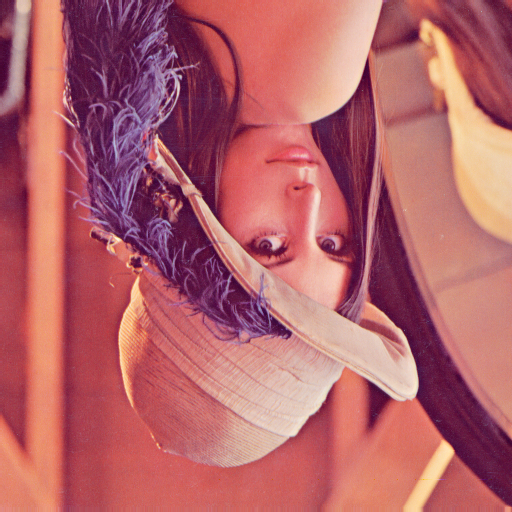
\includegraphics[width=8em]{image/Lenna_flip_vertical.png}} \\ \hline 
  5 & Chuyển đổi thành ảnh xám & 100\% & \parbox[c]{8em}{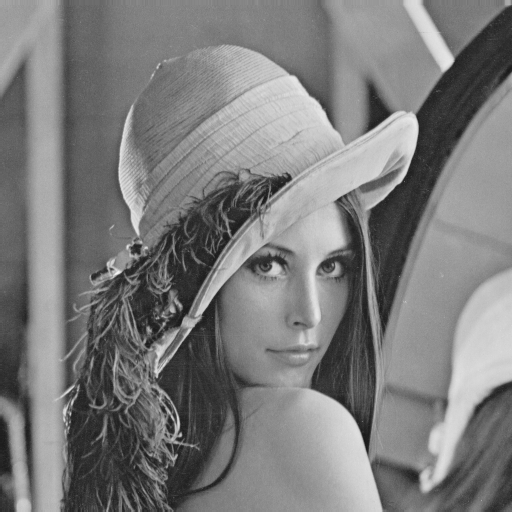
\includegraphics[width=8em]{image/Lenna_grayscale.png}} \\ \hline
  6 & Chuyển đổi thành ảnh sepia & 100\% & \parbox[c]{8em}{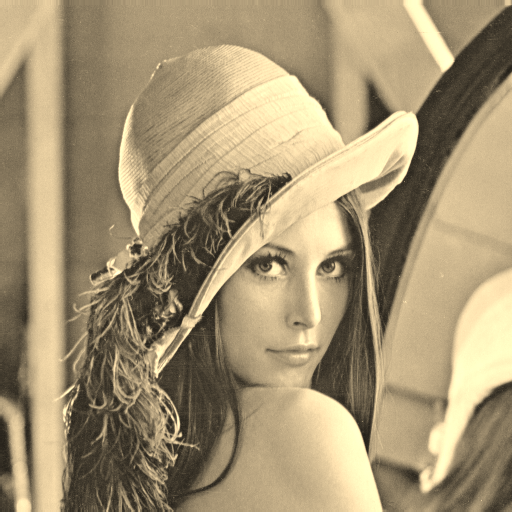
\includegraphics[width=8em]{image/Lenna_sepia.png}} \\ \hline
  7 & Làm mờ & 100\% & \parbox[c]{8em}{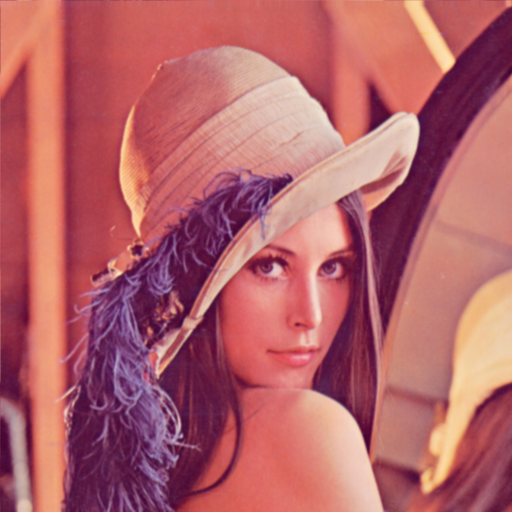
\includegraphics[width=8em]{image/Lenna_blur.png}} \\ \hline
  8 & Làm sắc nét ảnh & 100\% & \parbox[c]{8em}{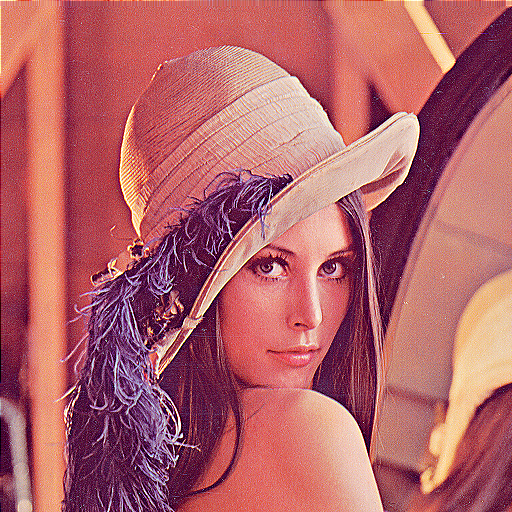
\includegraphics[width=8em]{image/Lenna_sharpen.png}} \\ \hline
  9 & Cắt ảnh theo kích thước (cắt ở trung tâm) & 100\% & \parbox[c]{8em}{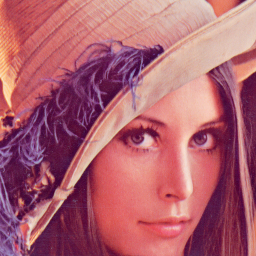
\includegraphics[width=8em]{image/Lenna_center_crop.png}} \\ \hline
  10 & Cắt ảnh theo khung hình tròn & 100\% & \parbox[c]{8em}{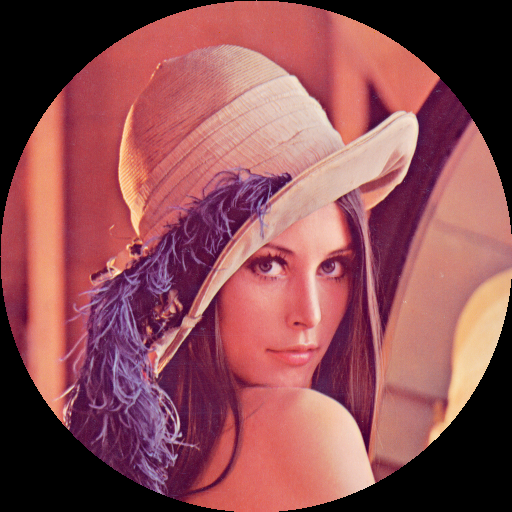
\includegraphics[width=8em]{image/Lenna_circular_crop.png}} \\ \hline
  11 & Cắt ảnh theo khung elip & 100\% & \parbox[c]{8em}{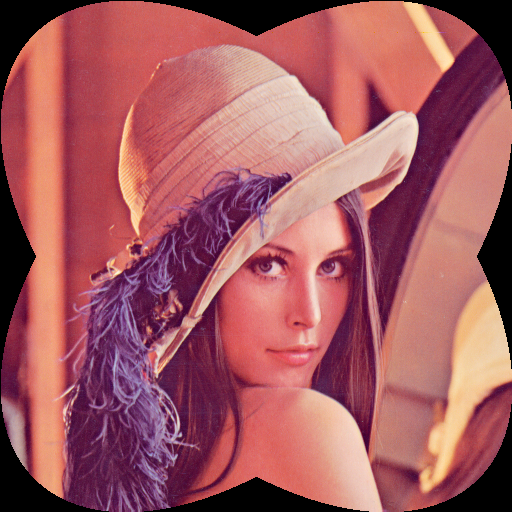
\includegraphics[width=8em]{image/Lenna_elliptical_crop.png}} \\ \hline
\end{longtable}

% \begin{table}[ht] 
%   \centering
%   \begin{tabular}{|l|l|l|l|l|} \hline 
%       Stimuli Category & Familiar Organism & Growth Model & Metamorphosis & Figure \\ \hline
%       \textbf{FDM} & Yes & Dramatic & Yes & \parbox[c]{7em}{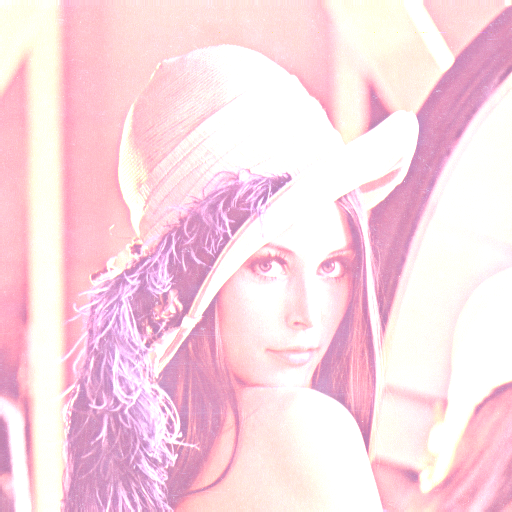
\includegraphics[width=0.15\textwidth]{image/Lenna_brightness_128.png}} \\ \hline
%   \end{tabular}
% \end{table}

\section{Mô tả}
\textcolor{red}{Để thuận tiện cho phần trình bày bên dưới, từ bây giờ, mỗi điểm ảnh gồm 3 giá trị của kênh màu RGB sẽ được xem như một phần tử màu. Do đó, ma trận các điểm ảnh được xem như mảng 2 chiều các điểm ảnh, kí hiệu: \textit{img\_2d}. }
% Template mô tả hàm
% \textbf{Input:} \\
% \textbf{Output:}
% \paragraph{Ý tưởng thực hiện:}
% \paragraph{Mô tả:}
\subsection{Nhóm hàm chính}
\subsubsection{Hàm change\_brightness}
\textbf{Input:} Mảng NumPy 2 chiều các điểm ảnh \textit{img\_2d}, giá trị độ sáng \textit{brightness} (mặc định là 128 nếu không truyền tham số vào hàm). \\
\textbf{Output:} Mảng NumPy 2 chiều các điểm ảnh, chuỗi kí tự chứa hậu tố của tên file ảnh sau xử lý.

\paragraph{Ý tưởng thực hiện:} Thay đổi độ sáng bức ảnh là cùng lúc thay đổi giá trị trong phần tử màu của từng pixel ảnh cho một hằng số. \\
Xét một pixel ảnh $p$ thuộc hệ màu RGB, giá trị của từng kênh màu là $[p_{1}, p_{2}, p_{3}]$. Giá trị của pixel ảnh $p$ sau khi thay đổi độ sáng được tính bằng công thức: 
\[[p_{1} + k , p_{2} + k, p_{3} + k]\]
với $k$ là hằng số thay đổi độ sáng. \\ Bức ảnh sau khi thay đổi độ sáng sẽ có màu sáng hơn hoặc tối hơn tùy thuộc vào giá trị của hằng số này, càng tối nghĩa là càng nhiều pixel có giá trị màu gần 0 và ngược lại.

\paragraph{Mô tả:} Để thay đổi độ sáng của ảnh, ta chỉ cần cộng thêm giá trị \textit{brightness} vào mỗi giá trị trong phần tử màu của mảng \textit{img\_2d}. Tuy nhiên, giá trị này có thể vượt quá khoảng giá trị cho phép của một giá trị của phần tử màu (từ 0 đến 255). Do đó, trước khi thực hiện phép cộng, ta cần đổi kiểu dữ liệu của mảng \textit{img\_2d} thành int64 để có thể lưu được các giá trị nguyên âm và giá trị nguyên dương lớn hơn 255. Sau khi thực hiện xong, kết hợp việc giới hạn giá trị sử dụng hàm \textit{limit\_value} và ép kiểu dữ liệu về uint8, ta được mảng 2 chiều các điểm ảnh sau khi thay đổi độ sáng. Việc ép kiểu mảng trước khi thực hiện phép cộng nhằm đảm bảo từng giá trị màu trong mỗi pixel không bị sai lệch giá trị (256 sẽ trở về 0 nếu không ép kiểu về int64).

\subsubsection{Hàm change\_contrast}
\textbf{Input:} Mảng NumPy 2 chiều các điểm ảnh \textit{img\_2d}, giá trị tương phản \textit{contrast} (mặc định là 128 nếu không truyền tham số vào hàm). \\
\textbf{Output:} Mảng NumPy 2 chiều các điểm ảnh, chuỗi kí tự chứa hậu tố của tên file ảnh sau xử lý.

\paragraph{Ý tưởng thực hiện:} Tương tự như việc thay đổi độ sáng của bức ảnh, thay đổi độ tương phản của bức ảnh là cùng lúc thay đổi giá trị trong phần tử màu của từng pixel ảnh cho một hằng số. Thay vì phép cộng như thay đổi độ sáng, giá trị của một phần tử màu thay đổi theo công thức:
\[ \text{R'} = \text{F} \times (\text{R}-128) + 128 \]
với:
\begin{itemize}
    \item \textit{R'} là giá trị của phần tử màu sau khi thay đổi độ tương phản.
    \item \textit{R} là giá trị của phần tử màu trước khi thay đổi độ tương phản.
    \item \textit{F} là hằng số thay đổi độ tương phản. Với \textit{C} là giá trị tương phản truyền vào hàm thì công thức của hằng số này:
    \[ \text{F} = \frac{259(\text{C}+255)}{255(259-\text{C})} \]
\end{itemize}

\paragraph{Mô tả:} Do \textit{F} được tính bởi công thức trên nên giá trị của \textit{F} có thể vượt quá 1, kéo theo đó, giá trị của mảng \textit{img\_2d} có thể vượt quá khoảng giá trị cho phép của một giá trị của phần tử màu (từ 0 đến 255). Do đó, trước khi thực hiện phép nhân, ta cần đổi kiểu dữ liệu của mảng \textit{img\_2d} thành float64 để có thể lưu được các giá trị số thực nhỏ hơn 0 và lớn hơn 255. Sau khi thực hiện xong, kết hợp việc giới hạn giá trị sử dụng hàm \textit{limit\_value} và ép kiểu dữ liệu về uint8, ta được mảng 2 chiều các điểm ảnh sau khi thay đổi độ tương phản.

\subsubsection{Hàm flip\_image}
\textbf{Input:} Mảng NumPy 2 chiều các điểm ảnh \textit{img\_2d}, hướng lật cần xử lý \textit{axis}. \\
\textbf{Output:} Mảng NumPy 2 chiều các điểm ảnh đã được lật theo hướng \textit{axis}, chuỗi kí tự chứa hậu tố của tên file ảnh sau xử lý.

\paragraph{Ý tưởng thực hiện:} Để lật ảnh theo chiều dọc, ta chỉ cần đảo ngược thứ tự các hàng của mảng \textit{img\_2d}, tương tự, để lật ảnh theo chiều ngang, ta chỉ cần đảo ngược thứ tự các cột của mảng. Để thực hiện được việc đảo ngược thứ tự các hàng hoặc cột của mảng mà không sử dụng hàm có sẵn của thư viện NumPy, ta sẽ sử dụng kỹ thuật slicing của Python.

\paragraph{Mô tả:} Trong hàm flip\_image, giá trị 0 và 1 được sử dụng để chỉ định trục mà hình ảnh sẽ được lật. Trong trường hợp này, giá trị 0 được sử dụng để chỉ định trục dọc (trục y) và giá trị 1 được sử dụng để chỉ định trục ngang (trục x), cách đánh số này phù hợp với cách đánh số các trục khi trục dọc được đánh số là trục thứ nhất và trục ngang được đánh số là trục thứ hai.
\begin{itemize}
  \item img\_2d[::-1, :]:
  Cú pháp này sẽ lấy toàn bộ các hàng của mảng \textit{img\_2d} nhưng đảo ngược thứ tự của chúng. Điều này có nghĩa là hàng đầu tiên sẽ trở thành hàng cuối cùng, hàng thứ hai sẽ trở thành hàng áp chót, và ngược lại. Kết quả thu được là một mảng mới với cùng kích thước như mảng ban đầu nhưng được lật theo chiều dọc.
  \item img\_2d[:, ::-1]:
  Cú pháp này sẽ lấy toàn bộ các cột của mảng \textit{img\_2d} nhưng đảo ngược thứ tự của chúng. Kết quả thu được là một mảng mới với cùng kích thước như mảng ban đầu nhưng được lật theo chiều ngang.
\end{itemize}
Dù lấy toàn bộ hàng hay cột của mảng thì phần tử màu của ảnh vẫn được giữ nguyên, chỉ thứ tự của chúng bị đảo ngược, do đó ở chiều thứ ba của mảng ảnh, ta không cần thực hiện việc slicing.

\subsubsection{Hàm convert\_grayscale}
\textbf{Input:} Mảng NumPy 2 chiều các điểm ảnh \textit{img\_2d}. \\
\textbf{Output:} Mảng NumPy 2 chiều các điểm ảnh đã được chuyển sang ảnh xám, chuỗi kí tự chứa hậu tố của tên file ảnh sau xử lý.

\paragraph{Ý tưởng thực hiện:} Để chuyển ảnh màu sang ảnh xám, ta sẽ sử dụng công thức sau (luminosity method):
\[ \text{Y} = 0.3*\text{R} + 0.59*\text{G} + 0.11*\text{B}\]
Trong đó, R, G, B lần lượt là giá trị của các phần tử màu Red, Green, Blue của điểm ảnh đang xét. Sau khi tính được giá trị Y, ta sẽ gán giá trị Y cho cả 3 phần tử màu của điểm ảnh đang xét. Và một cách dễ hình dung, ta nhân vô hướng vector [R, G, B] của từng điểm ảnh với vector [0.3, 0.59, 0.11] để tính được giá trị Y. Để thực hiện được việc nhân vô hướng này, ta sẽ sử dụng hàm dot của thư viện NumPy.

Cần lưu ý rằng tích vô hướng của 2 vector là một số (scalar), nhưng mỗi điểm ảnh trong bức ảnh cần 3 kênh màu (với hệ màu RGB), ta cần lặp lại giá trị Y 3 lần để gán cho điểm ảnh đang xét. Để thực hiện việc lặp lại này, ta sẽ sử dụng hàm repeat của thư viện NumPy. Trong trường hợp này, ta sẽ lặp lại giá trị Y của các điểm ảnh 3 lần theo trục cuối cùng (\textit{axis=-1}).

\paragraph{Mô tả:}
Đối với hàm NumPy dot \textcolor{red}{\textit{numpy.dot(a, b, out=None)}}, nếu a là mảng nhiều chiều và b là mảng một chiều thì kết quả là tích vô hướng trên trục cuối cùng của a và b. Tận dụng đặc tính này của hàm, ta sẽ nhân vô hướng mảng \textit{img\_2d} với mảng 1 chiều [0.3, 0.59, 0.11]. Do trục cuối cùng của mảng \textit{img\_2d} là mảng 1 chiều chứa giá trị của 3 phần tử màu của điểm ảnh, nên kết quả thu được là mảng 2 chiều chứa giá trị Y của các điểm ảnh (\textit{gray\_image}). 

Tham số cần truyền vào hàm repeat lần lượt là mảng chứa các giá trị cần lặp lại, số lần lặp lại (\textit{repeats}), và trục cần lặp lại (\textit{axis}). Mảng \textit{gray\_image} đang là mảng 2 chiều chứa giá trị Y của các điểm ảnh, ta sẽ mở rộng mảng này thêm 1 chiều ở trục cuối cùng bằng cách sử dụng \textit{gray\_image[...,None]}, sau đó lặp lại mảng này 3 lần (một cách tổng quát hơn là \textit{img\_2d.shape[-1]} lần) theo trục cuối cùng (\textit{axis=-1}). Với công thức chuyển đổi ảnh xám sử dụng luminosity method như trên, giá trị Y đảm bảo hợp lệ nên ta không cần thực hiện việc giới hạn giá trị cũng như ép kiểu kết quả thu được.

\subsubsection{Hàm convert\_sepia}
\textbf{Input:} Mảng NumPy 2 chiều các điểm ảnh \textit{img\_2d}. \\
\textbf{Output:} Mảng NumPy 2 chiều các điểm ảnh đã được chuyển sang ảnh sepia, chuỗi kí tự chứa hậu tố của tên file ảnh sau xử lý.

\paragraph{Ý tưởng thực hiện:} Để chuyển ảnh màu sang ảnh sepia, ta sẽ sử dụng công thức sau:
\begin{align*}
  \text{newRed} = 0.393*\text{R} + 0.769*\text{G} + 0.189*\text{B} \\
  \text{newGreen} = 0.349*\text{R} + 0.686*\text{G} + 0.168*\text{B} \\
  \text{newBlue} = 0.272*\text{R} + 0.534*\text{G} + 0.131*\text{B} 
\end{align*}
với R, G, B lần lượt là giá trị của các phần tử màu Red, Green, Blue của điểm ảnh đang xét. Sau khi tính được giá trị newRed, newGreen, newBlue, ta lần lượt gán các giá trị trên vào các điểm ảnh. \\
Xét một pixel ảnh $p$ thuộc hệ màu RGB, giá trị của từng kênh màu là $[p_{1}, p_{2}, p_{3}]$. Ta có thể viết lại công thức trên dưới dạng ma trận như sau:
\begin{align*}
  \begin{bmatrix}
    \text{newRed} \\
    \text{newGreen} \\
    \text{newBlue}
  \end{bmatrix}
  =
  \begin{bmatrix}
    0.393 & 0.769 & 0.189 \\
    0.349 & 0.686 & 0.168 \\
    0.272 & 0.534 & 0.131
  \end{bmatrix}
  \begin{bmatrix}
    p_{1} \\
    p_{2} \\
    p_{3}
  \end{bmatrix}
\end{align*}
$\Leftrightarrow$
\begin{align*}
  \begin{bmatrix}
    \text{newRed} & \text{newGreen} & \text{newBlue}
  \end{bmatrix}
  =
  \begin{bmatrix}
    p_{1} & p_{2} & p_{3}
  \end{bmatrix}
  \begin{bmatrix}
    0.393 & 0.769 & 0.189 \\
    0.349 & 0.686 & 0.168 \\
    0.272 & 0.534 & 0.131
  \end{bmatrix}^\top
\end{align*}
Bằng việc ma trận hoá công thức trên, ta dễ dàng sử dụng hàm dot trong thư viện NumPy để thực hiện tính toán. Cần lưu ý rằng với trọng số như trên, các giá trị của phần tử màu có thể vượt quá giá trị cho phép của kiểu dữ liệu uint8 nên cần giới hạn giá trị của kết quả trả về.

\paragraph{Mô tả:}
Đối với hàm \textcolor{red}{np.dot(a, b, out=None)}, nếu a là một mảng nhiều chiều và b là một mảng hai chiều thì kết quả là tích vô hướng trên từng phần tử trên trục cuối cùng của a với trục gần cuối của b.\\
Do trục cuối cùng của mảng \textit{img\_2d} là mảng 1 chiều chứa 3 phần tử màu của điểm ảnh và trục gần cuối của ma trận chuyển vị của mảng \textit{sepia\_array} có giá trị là các hàng của mảng \textit{sepia\_array.T}, là trọng số của các kênh màu Red, Green, Blue trong công thức chuyển đổi ảnh màu sang ảnh sepia, nên kết quả của phép nhân này chính là giá trị của các kênh màu mới của điểm ảnh.\\
Với trọng số như trên, các giá trị của phần tử màu có thể vượt quá giá trị cho phép của kiểu dữ liệu uint8 nên cần giới hạn giá trị của kết quả trả về bằng hàm \textit{limit\_value}.

\subsubsection{Hàm convolute\_2D}
\subsubsection{Hàm blur\_image / sharpen\_image}

\subsubsection{Hàm center\_crop}
\textbf{Input:} Mảng NumPy 2 chiều các điểm ảnh \textit{img\_2d}, kích thước chiều cao \textit{height} và chiều rộng \textit{width} của ảnh đầu ra (mặc định kích thước ảnh đầu ra là 256x256 nếu ta không truyền 2 tham số này vào hàm). \\
\textbf{Output:} Mảng NumPy 2 chiều các điểm ảnh \textit{img\_2d} đã được cắt trung tâm theo kích thước \textit{height} và \textit{width}, và chuỗi kí tự chứa hậu tố của tên file ảnh đầu ra. \\
\paragraph{Ý tưởng thực hiện:} Với yêu cầu cắt ảnh từ trung tâm, ta cần xác định vị trí của pixel đầu tiên của ảnh đầu ra. Toạ độ của pixel đầu tiên của ảnh đầu ra (tạm gọi (\text{x\_{start}}, \text{y\_{start}})) được thể hiện như trên hình:
\begin{figure}[!ht]
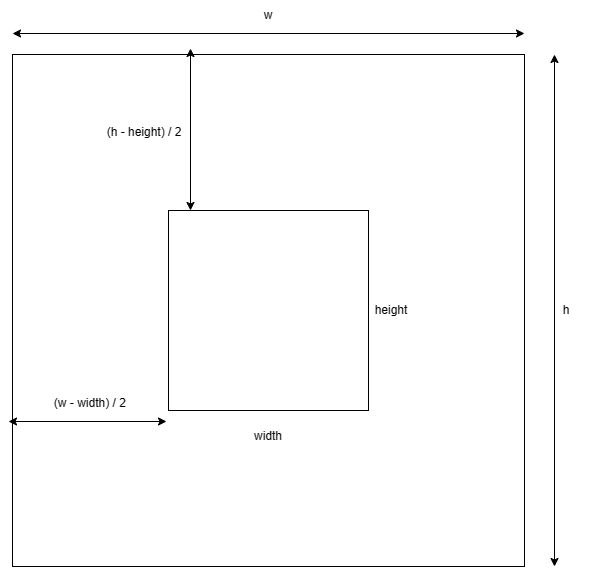
\includegraphics[width = .5\textwidth]{image/square_center.png}
\end{figure} \\
Từ vị trí \text{x\_{start}}, \text{y\_{start}} trên, ta có thể xác định vị trí của pixel cuối cùng của ảnh đầu ra (tạm gọi (\text{x\_{end}}, \text{y\_{end}})) như sau:
\begin{align*}
  \begin{cases}
    \text{x\_{end}} = \text{x\_{start}} + \text{height} \\
    \text{y\_{end}} = \text{y\_{start}} + \text{width}
  \end{cases}
\end{align*}
Với \textit{height} và \textit{width} là kích thước của ảnh đầu ra. \\
Sau khi xác định được vị trí của pixel đầu tiên và pixel cuối cùng của ảnh đầu ra, ta có thể cắt ảnh đầu vào theo vị trí này để được ảnh đầu ra bằng kỹ thuật slicing. 

\paragraph{Mô tả:}


\subsubsection{Hàm circular\_crop}
\subsubsection{Hàm elliptical\_crop}

\subsection{Nhóm hàm bổ trợ}
\subsubsection{Hàm limit\_value}
\subsubsection{Hàm show\_image}
\subsubsection{Hàm write\_image}
\subsubsection{Hàm read\_image}
\subsubsection{Hàm main}

\newpage
\subsection{Nhận xét}
\subsubsection{Về ảnh đầu ra}

\subsubsection{Về tài nguyên sử dụng}

\centerline{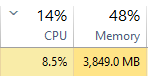
\includegraphics[width=0.2\textwidth]{image/performance.png}}
\newpage
\section{Tài liệu tham khảo}
\begin{itemize}
  \item Brightness
  \begin{enumerate}
    \item \href{https://ie.nitk.ac.in/blog/2020/01/19/algorithms-for-adjusting-brightness-and-contrast-of-an-image/}{Algorithms for adjusting brightness and contrast of an image}
  \end{enumerate}
  \item Contrast
  \begin{enumerate}
      \item \href{https://www.dfstudios.co.uk/articles/programming/image-programming-algorithms/image-processing-algorithms-part-5-contrast-adjustment/}{Image Processing Algorithms Part 5 - Contrast Adjustment}
  \end{enumerate}
  \item Flip
  \begin{enumerate}
      \item \href{https://www.w3schools.com/python/numpy/numpy_array_slicing.asp}{NumPy Array Slicing}
  \end{enumerate}
  \item Grayscale/Sepia Conversion
  \begin{enumerate}
    \item \href{https://www.tutorialspoint.com/dip/grayscale_to_rgb_conversion.htm}{Convert RGB to Grayscale}
    \item \href{https://www.geeksforgeeks.org/image-processing-in-java-colored-image-to-sepia-image-conversion/}{Convert RGB to Sepia}
    \item \href{https://numpy.org/doc/stable/reference/generated/numpy.dot.html}{NumPy dot}
    \item \href{https://numpy.org/doc/stable/reference/generated/numpy.repeat.html}{NumPy repeat}
  \end{enumerate} 
\end{itemize}

\end{document}